\documentclass[a4paper,12pt,oneside]{book}
\usepackage{graphicx}
\usepackage{hyperref}
\usepackage[T1]{fontenc}
\usepackage[utf8]{inputenc}
\usepackage{setspace}
\usepackage[paper=a4paper,margin=1in]{geometry}
\usepackage{imakeidx}
\usepackage{amsmath}
\usepackage{amssymb}
\usepackage{algorithm}
\usepackage{algpseudocode}

\makeindex

\begin{document}
    
    \begin{titlepage}
        
	\vspace{40mm}
        
	\begin{center}
            {\LARGE{
                    \setstretch{1.2}
                    \textbf{Appunti di \\ Ingegneria del Software}
                    \par
            }}
        \end{center}
        
        \vspace{50mm}

        \begin{flushright}
            {\large \textbf{A cura di:}} \\
            \large{Francesco Refolli} \\
            \large{Matricola 865955} 
        \end{flushright}
        
        \vspace{40mm}
        \begin{center}
            {\large{\bf Anno Accademico 2022-2023}}
        \end{center}

        \restoregeometry
        
    \end{titlepage}
    
    \printindex
    
    \part{Architectural Patterns}
    \chapter{Lazy Load}

\section{Descrizione}

"An object that doesn’t contain all of the data you need but knows how to get it" - Martin Fowler

Quando una Classe deve mantenere memorizzati dei dati, e' utile che essi siano caricati tanto tardi quanto e' bassa la probabilita' che si ricorra ad essi.
Ovvero si rimanda il caricamento dei dati alla prima occorrenza di utilizzo.
Per ottenere questo e' necessario che essa possa ottenere o popolare i dati che gli spettano.

\section{Vista UML}

\begin{center}
    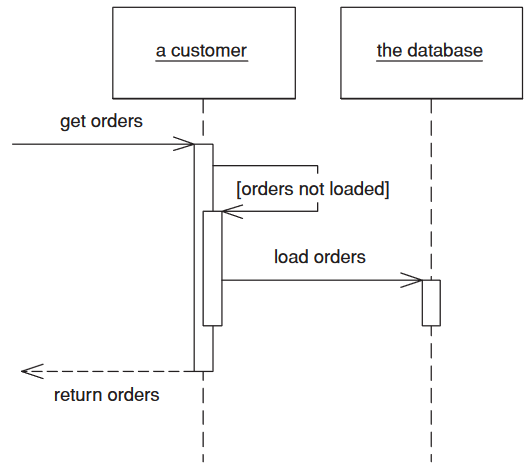
\includegraphics[width=12cm]{images/lazy-load/LazyLoad.png}
\end{center}

\section{Vantaggi}

Il vantaggio principale riguarda le prestazioni e in particolare la velocita' con cui una classe o istanza viene caricata in memoria.
Se meno dati vengono precaricati (perche' al momento inutili) allora minore sara' il carico di lavoro dei calcolatori che la elaborano.
Inoltre se l'istanza verra' eliminata dalla memoria senza che quei dati vengano acceduti, sara' possibile risparmiare anche sul tempo di eliminazione dei dati.
Bisogna altresi' considerare che questo determina anche un uso piu' ottimizzato della memoria: per tutto il tempo in cui non sara' necessaria la risorsa A, ci sara' piu' spazio in memoria per utilizzare il resto delle risorse.

\section{Svantaggi}

Si supponga ora che la classe abbia come responsabilita' la manipolazione dei dati e il caricamento lazy degli stessi.
Il Single Responsibility Principle prescrive che ogni classe abbia solo una responsabilita', in modo tale che abbia meno motivi possibili per diventare obsoleta.
Se si vuole rispettare questo principio occorre esportare la responsabilita' di caricamento lazy ad una classe di supporto.
Questo pero' genera necessariamente accoppiamento a seguito di questa nuova dipendenza.
E' quindi essenziale effettuare una scelta ponderata che tenga conto delle priorita'.

\section{Quando Usarlo}

Questa strategia e' utile quando i dati non sono immediatamente necessari per l'elaborazione e quando per recuperarli servono molteplici operazioni rimandabili.
Quando una operazione deve essere fatta e' utile caricare tutti i dati che essa possa caricare per evitare di doverla ripetere. E' quindi consigliato evitare di inserire Lazy Load multipli a meno che non si tratti di dati eterogenei e ulteriormente rimandabili.
Quando si vuole gestire dall'interno una inizializzazione onerosa e complessa e' di norma possibile applicare senza troppi problemi questo pattern per articolare questa fase senza sbilanciare il carico dell'applicativo.

    \chapter{Lazy Load}

\section{Descrizione}

"An object that doesn’t contain all of the data you need but knows how to get it" - Martin Fowler

Quando una Classe deve mantenere memorizzati dei dati, e' utile che essi siano caricati tanto tardi quanto e' bassa la probabilita' che si ricorra ad essi.
Ovvero si rimanda il caricamento dei dati alla prima occorrenza di utilizzo.
Per ottenere questo e' necessario che essa possa ottenere o popolare i dati che gli spettano.

\section{Vista UML}

\begin{center}
    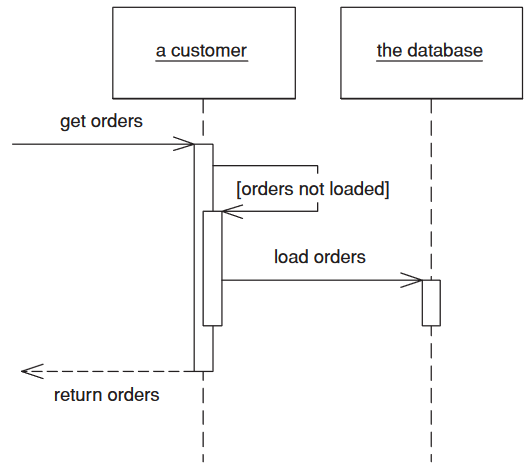
\includegraphics[width=12cm]{images/lazy-load/LazyLoad.png}
\end{center}

\section{Vantaggi}

Il vantaggio principale riguarda le prestazioni e in particolare la velocita' con cui una classe o istanza viene caricata in memoria.
Se meno dati vengono precaricati (perche' al momento inutili) allora minore sara' il carico di lavoro dei calcolatori che la elaborano.
Inoltre se l'istanza verra' eliminata dalla memoria senza che quei dati vengano acceduti, sara' possibile risparmiare anche sul tempo di eliminazione dei dati.
Bisogna altresi' considerare che questo determina anche un uso piu' ottimizzato della memoria: per tutto il tempo in cui non sara' necessaria la risorsa A, ci sara' piu' spazio in memoria per utilizzare il resto delle risorse.

\section{Svantaggi}

Si supponga ora che la classe abbia come responsabilita' la manipolazione dei dati e il caricamento lazy degli stessi.
Il Single Responsibility Principle prescrive che ogni classe abbia solo una responsabilita', in modo tale che abbia meno motivi possibili per diventare obsoleta.
Se si vuole rispettare questo principio occorre esportare la responsabilita' di caricamento lazy ad una classe di supporto.
Questo pero' genera necessariamente accoppiamento a seguito di questa nuova dipendenza.
E' quindi essenziale effettuare una scelta ponderata che tenga conto delle priorita'.

\section{Quando Usarlo}

Questa strategia e' utile quando i dati non sono immediatamente necessari per l'elaborazione e quando per recuperarli servono molteplici operazioni rimandabili.
Quando una operazione deve essere fatta e' utile caricare tutti i dati che essa possa caricare per evitare di doverla ripetere. E' quindi consigliato evitare di inserire Lazy Load multipli a meno che non si tratti di dati eterogenei e ulteriormente rimandabili.
Quando si vuole gestire dall'interno una inizializzazione onerosa e complessa e' di norma possibile applicare senza troppi problemi questo pattern per articolare questa fase senza sbilanciare il carico dell'applicativo.


    \part{Architectural Patterns Applications}
    \chapter{Lazy Load}

Fowler fornisce quattro implementazioni per questo pattern.

\section{Lazy Inizialization}

\begin{center}
    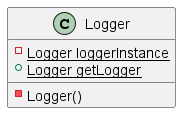
\includegraphics[width=12cm]{images/lazy-load/LoggerUML.png}
    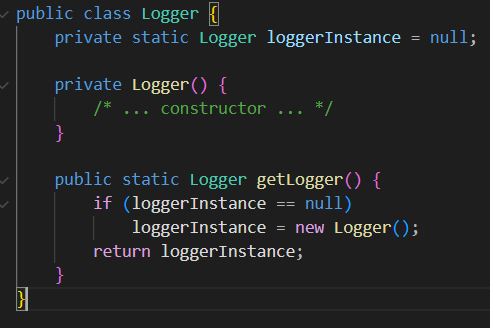
\includegraphics[width=12cm]{images/lazy-load/Logger.png}
\end{center}

In questa implementazione si controlla la disponibilita' del dato ed eventualmente si istanzia. Quindi viene ritornato.

\section{Virtual Proxy}

\begin{center}
    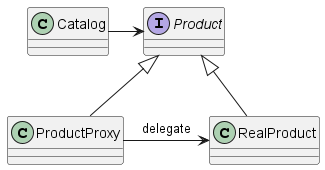
\includegraphics[width=12cm]{images/lazy-load/VirtualProxy.png}
\end{center}

Si crea una astrazione con una interfaccia e un intermediario che delega al RealProduct gli obiettivi di Product e si occupa soltanto di fornire all'occorrenza i servizi del RealProduct al Catalog.

\section{Value Holder}

\begin{center}
    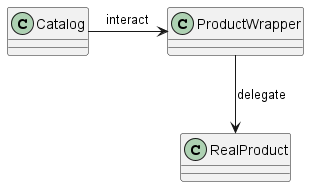
\includegraphics[width=12cm]{images/lazy-load/ValueHolder.png}
\end{center}

Si usa un ProductWrapper che assume tutte le responsabilita' che aveva il ProductProxy
La differenza con il Virtual Proxy e' che in questo caso il Catalog e' cosciente di stare interagendo con il ProductWrapper.

\section{Ghost}

\begin{center}
    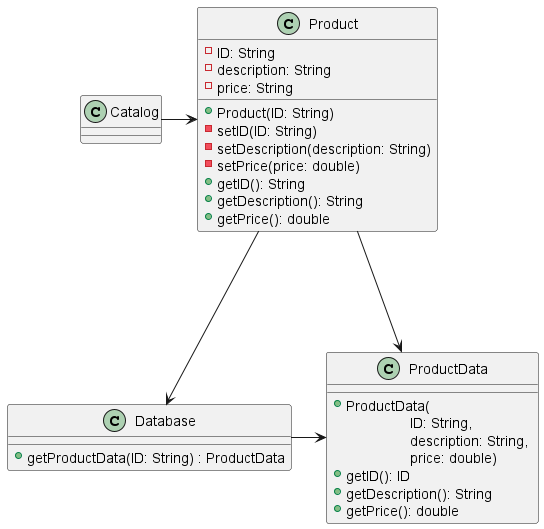
\includegraphics[width=12cm]{images/lazy-load/ProductClass.png}
    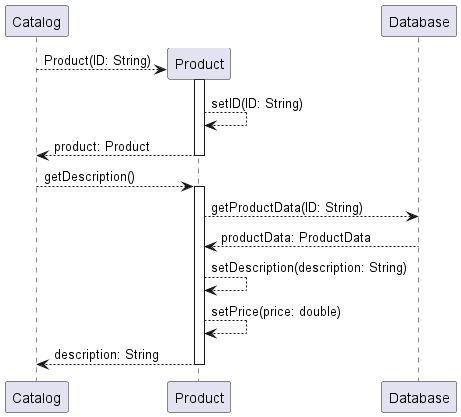
\includegraphics[width=12cm]{images/lazy-load/ProductSD.png}
\end{center}

Il Ghost qui' e' la classe Product, la quale e' un oggetto che quando viene instanziato contiene solo parte delle sue informazioni (ID), ma quando richiesto carica il resto delle informazioni.
Si noti che la classe ProductData e' immutabile, ed utilizzata solo per pattare informazioni tra il Database e il Product.

    \chapter{Lazy Load}

Fowler fornisce quattro implementazioni per questo pattern.

\section{Lazy Inizialization}

\begin{center}
    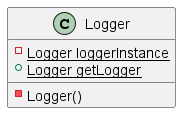
\includegraphics[width=12cm]{images/lazy-load/LoggerUML.png}
    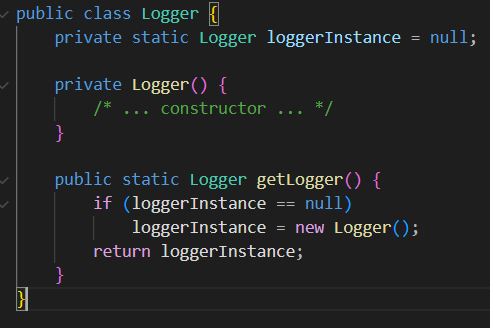
\includegraphics[width=12cm]{images/lazy-load/Logger.png}
\end{center}

In questa implementazione si controlla la disponibilita' del dato ed eventualmente si istanzia. Quindi viene ritornato.

\section{Virtual Proxy}

\begin{center}
    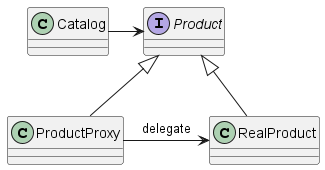
\includegraphics[width=12cm]{images/lazy-load/VirtualProxy.png}
\end{center}

Si crea una astrazione con una interfaccia e un intermediario che delega al RealProduct gli obiettivi di Product e si occupa soltanto di fornire all'occorrenza i servizi del RealProduct al Catalog.

\section{Value Holder}

\begin{center}
    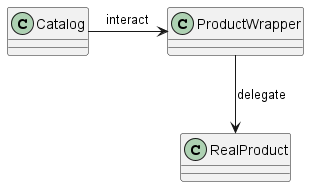
\includegraphics[width=12cm]{images/lazy-load/ValueHolder.png}
\end{center}

Si usa un ProductWrapper che assume tutte le responsabilita' che aveva il ProductProxy
La differenza con il Virtual Proxy e' che in questo caso il Catalog e' cosciente di stare interagendo con il ProductWrapper.

\section{Ghost}

\begin{center}
    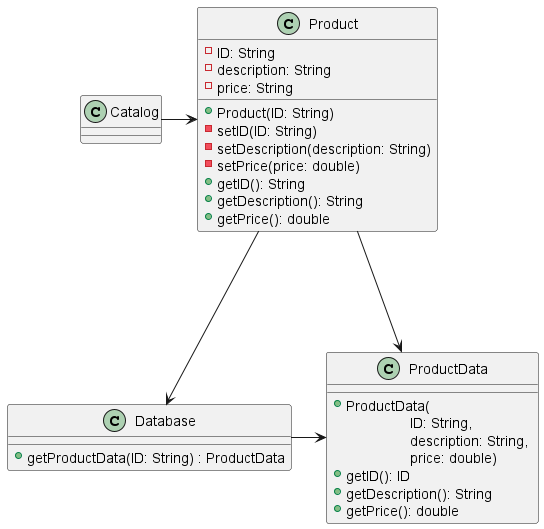
\includegraphics[width=12cm]{images/lazy-load/ProductClass.png}
    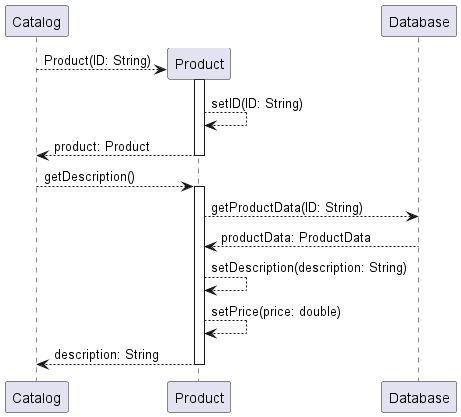
\includegraphics[width=12cm]{images/lazy-load/ProductSD.png}
\end{center}

Il Ghost qui' e' la classe Product, la quale e' un oggetto che quando viene instanziato contiene solo parte delle sue informazioni (ID), ma quando richiesto carica il resto delle informazioni.
Si noti che la classe ProductData e' immutabile, ed utilizzata solo per pattare informazioni tra il Database e il Product.

\end{document}
